\documentclass{article}
\usepackage{fullpage}
\usepackage[czech]{babel}
\usepackage{amsfonts}
\usepackage{fontawesome5}
\usepackage{hyperref}
\usepackage{graphicx}
\usepackage{caption}

\title{\vspace{-2cm}Franská říše (481 -- 843)\vspace{-1.7cm}}
\date{}

\begin{document}
\maketitle
\section*{Meroveovci 481 -- 751}
\begin{minipage}{0.6\textwidth}\raggedleft
    \begin{itemize}
        \setlength\itemsep{0.15em}
        \item[$-$] založena Franky, kteří sjednotili Germány
        \item[$-$] zakladatel \textbf{Chlodvík z Meroveovců} (481 -- 511)
            \begin{description}
                \vspace{-0.5em}
                \setlength\itemsep{0.15em}
                \item[497/98] nechal se pokřtít v Remeši\\
                $\rightarrow$ podporoval katolickou církev
                \item[$-$] \textit{Lex Salica} -- kodifikování práva
            \end{description}
        \vspace{-0.5em}
        \item[$-$] \textbf{Řehoř z Tours} -- mnich, napsal kroniku Franků (\textit{Historia Francorum})
        \item[$-$] \textbf{Dagobert I.} (629 -- 639)
            \vspace{-0.5em}
            \begin{description}
                \setlength\itemsep{0.15em}
                \item[631] \textsc{bitva u Wogastisburgu} vs. Sámova říše, (S. ř. vyhrává)
            \end{description}
        \vspace{-0.5em}
        \item[$-$] \uv{\textit{líní králové}} $\rightarrow$ \textit{majordomové} (správci paláců) na sebe strhávají moc $\rightarrow$  z nich dynastie Karlovců
        \item[$-$] \textbf{Pipin. II. Prostřední} (679 -- 714)
            \begin{description}
                \setlength\itemsep{0.15em}
                \vspace{-0.5em}
                \item[(687)] \textsc{bitva u Tertry}
            \end{description}
            \vspace{-0.5em}
        \item[$-$] \textbf{Karel Martell} (715 -- 741)
        \begin{description}
            \vspace{-0.5em}
            \setlength\itemsep{0.15em}
            \item[732] \textsc{bitva u Poitiers} a \textsc{bitva u Tours} -- zastavení postupu Arabů
        \end{description}
    \end{itemize}
\end{minipage}
\hfill
\noindent\begin{minipage}{0.3\textwidth}
    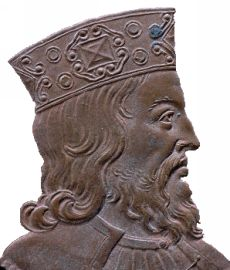
\includegraphics[width=\linewidth]{chlodvik.jpg}
    \captionof{figure}{Chlodvík z Meroveovců}
\end{minipage}

\section*{Karlovci 751 -- 843}
\begin{minipage}{0.6\textwidth}\raggedleft
    \begin{itemize}
        \setlength\itemsep{0.15em}
        \item[$-$] \textbf{Pipin III. Krátký}
        \begin{description}
            \vspace{-0.5em}
            \setlength\itemsep{0.15em}
            \item[751] prohlásil se za krále = \textit{rex francorum}, korunován papežem v Saint Denis
            \item[(755/6)] porážka Langobardů
        \end{description}
        \item[$-$] \textbf{Karel Veliký} (768 -- 814)
            \begin{description}
                \vspace{-0.5em}
                \setlength\itemsep{0.15em}
                \item[800] první císař (papež Lev III.)
                \item[$-$] definitivně poráží Langobardy v S Itálii
                \item[$-$] rozvoj kultury
                \item[Správa státu:] rozděleno na hrabství, v čele \textit{hrabata}, biskupství, v čele \textit{biskup}, v okrajových oblastech marka, v čele \textit{markrabě}
            \end{description}
        \end{itemize}
\end{minipage}
\hfill
\noindent\begin{minipage}{0.3\textwidth}
    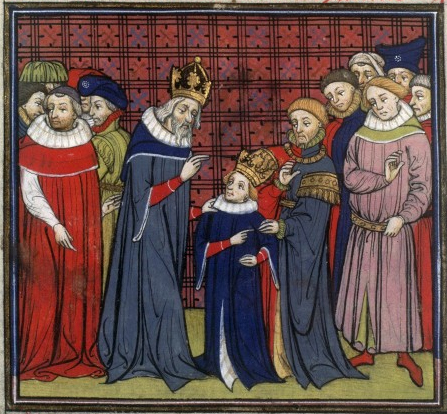
\includegraphics[width=\linewidth]{kv.jpg}
    \captionof{figure}{Karel Veliký a jeho syn Ludvík Pobožný}
\end{minipage}

\begin{minipage}{0.6\textwidth}\raggedleft
    \begin{itemize}
        \setlength\itemsep{0.15em}
        \item[$-$] \textit{karolínská renesance} -- podpora vzdělanosti a vědy, opět antické ideály
        \item[$-$] mnich \textbf{Alcuin z Yorku} (\href{https://cs.wikipedia.org/wiki/Alcuin}{\faWikipediaW ikipedie})
        \item[$-$] historik \textbf{Pavel Diaconus} (\href{https://cs.wikipedia.org/wiki/Paulus_Diaconus}{\faWikipediaW ikipedie})
        \item[$-$] Petr Pisánský
        \item[$-$] Einhard: \textit{Vita Karoli Magni} (\href{https://cs.wikipedia.org/wiki/Vita_Karoli_Magni}{\faWikipediaW ikipedie})
        \item[$-$] sídlo v Cáchách -- kaple Panny  Marie
        \item[$-$] \textbf{Ludvík Pobožný} (814 -- 840), 3 synové, chce mezi ně rozdělit říši = \textit{ordinatio imperii}
    \end{itemize}
\end{minipage}
\hfill
\noindent\begin{minipage}{0.3\textwidth}
    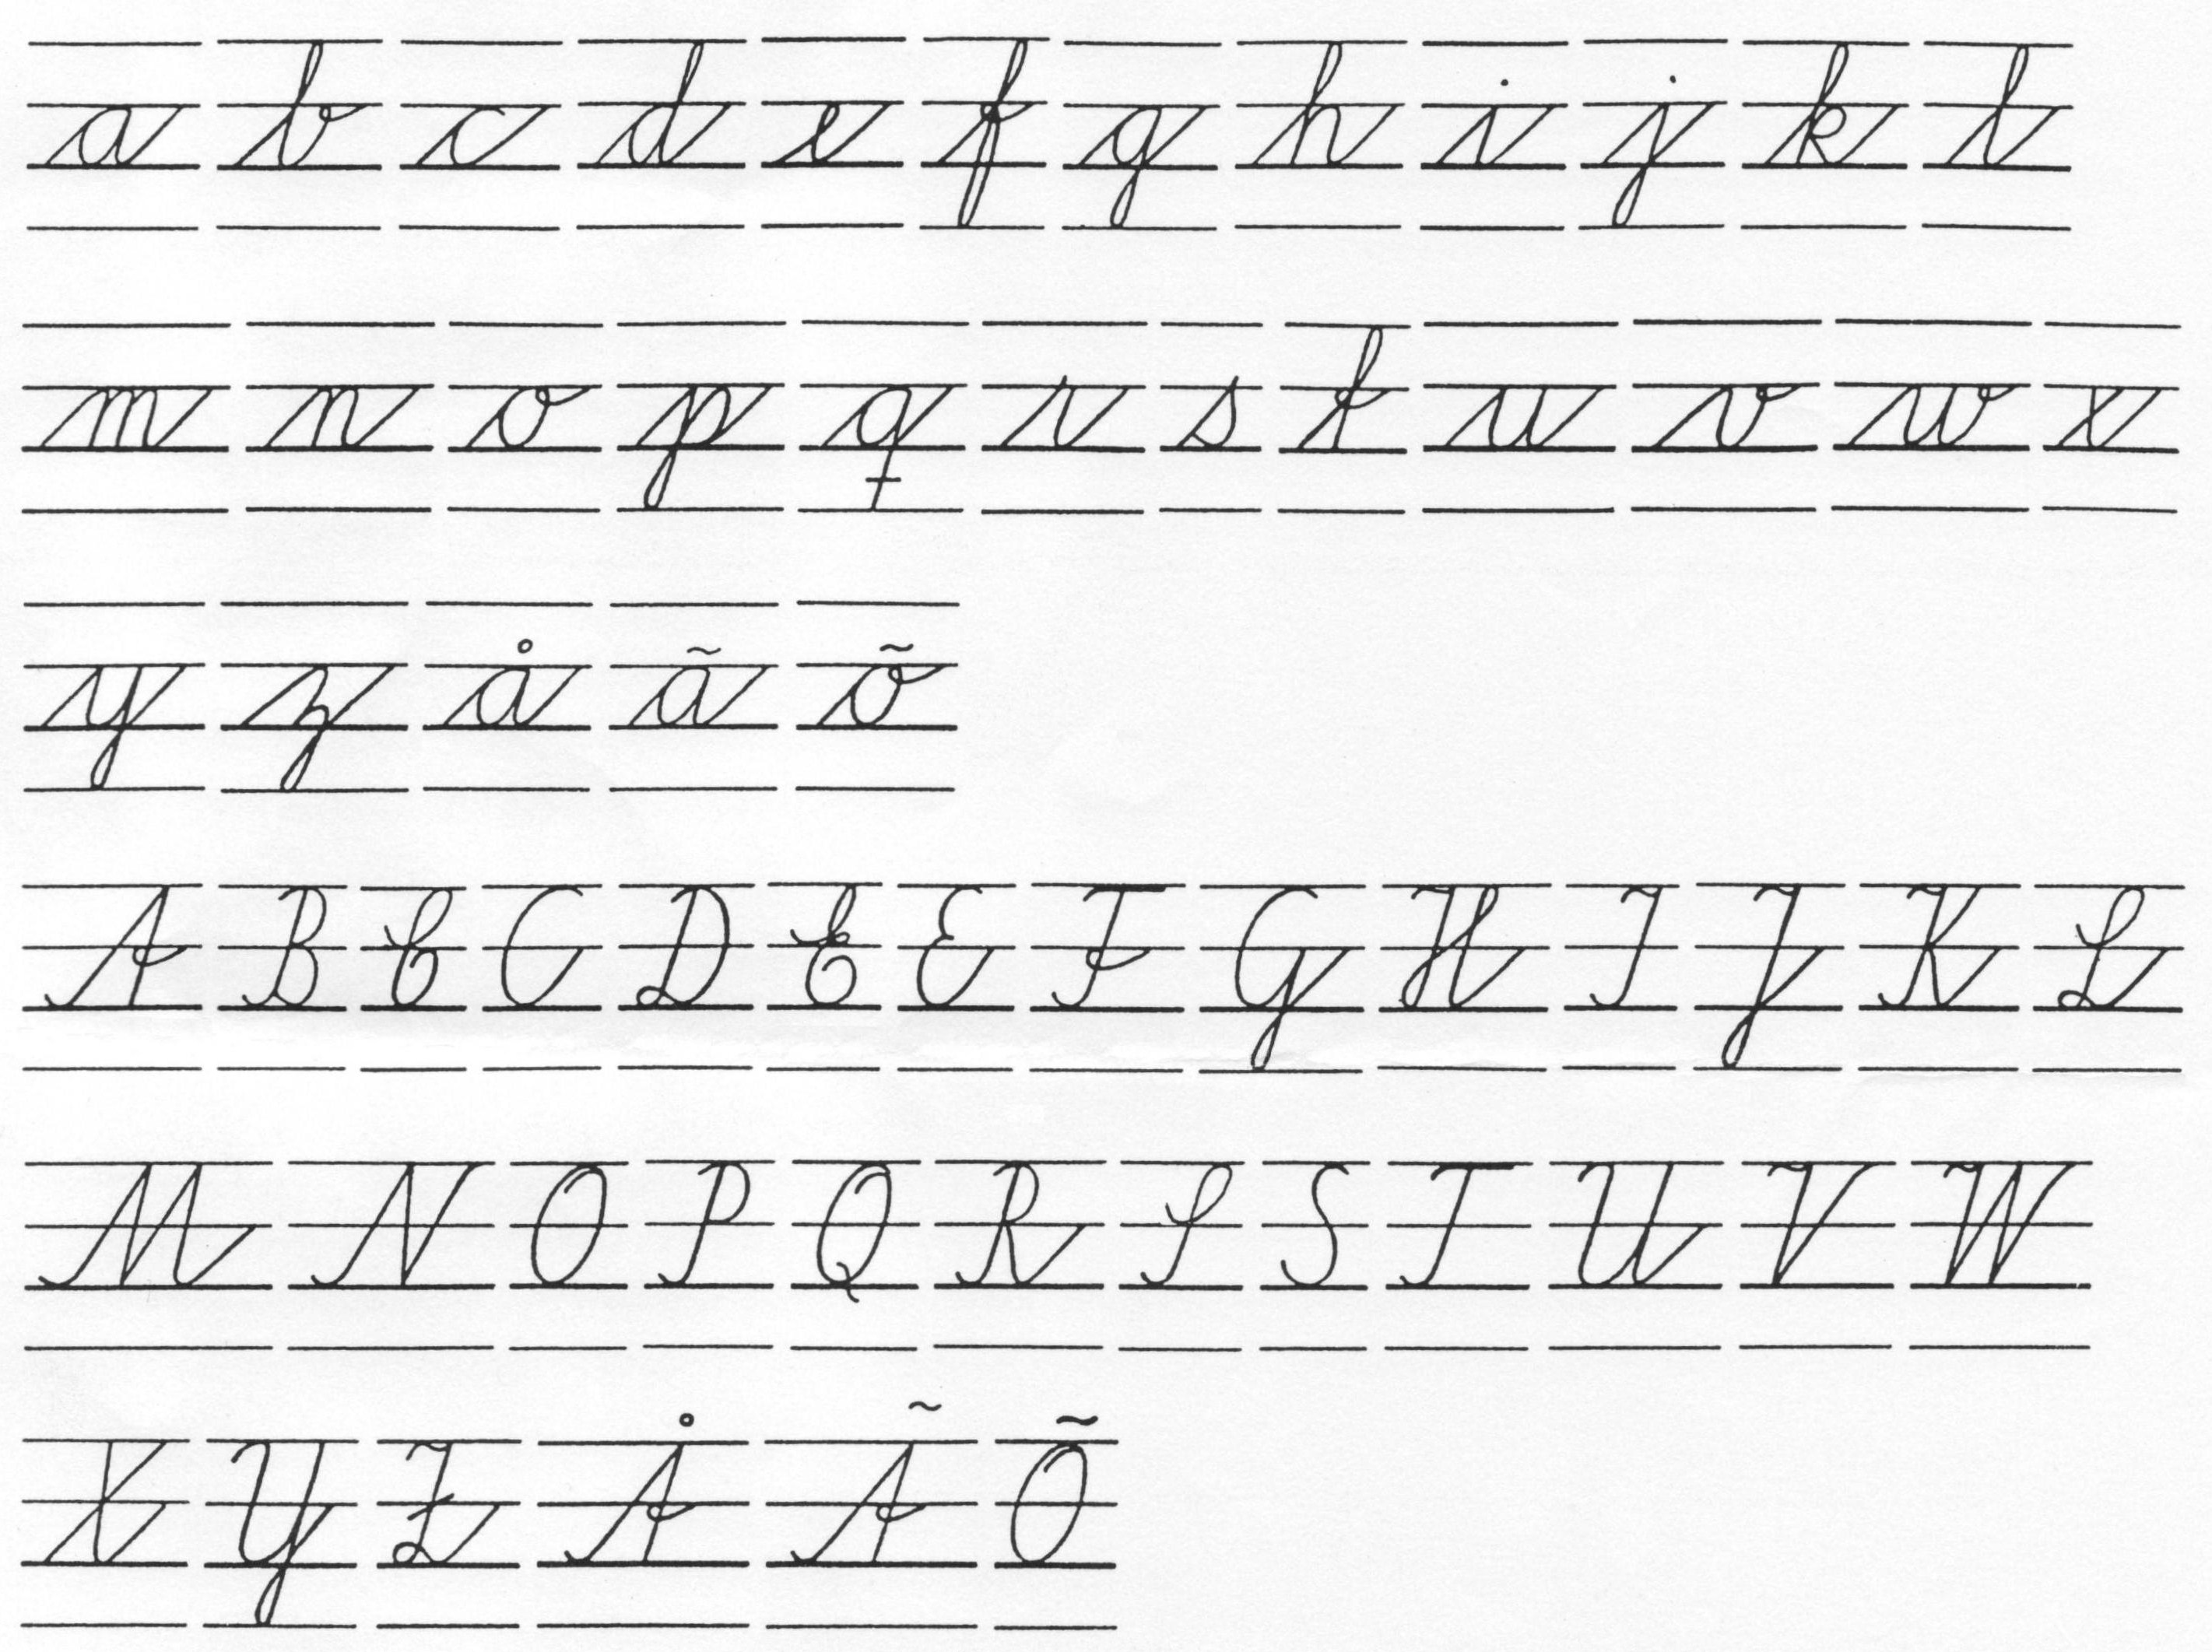
\includegraphics[width=\linewidth]{miniskule.jpg}
    \captionof{figure}{\textit{Miniskule} (nahoře) a majuskule (dole)}
\end{minipage}


\section*{Zánik Franské říše}
\begin{description}
    \setlength\itemsep{0.15em}
    \item[817] \textit{ordinatio imperii}
    \item[843] \textbf{Verdunská smlouva} -- rozdělení říše na Z $\rightarrow$ Francie, V $\rightarrow$ SŘŘ
    \item[Lothar I.] titul císaře, území: S Apeninského pol.
    \item[Karel II. Holý] Západofranská říše -- Francie
    \item[Ludvík II. Němec] Svatá říše římská
\end{description}

\begin{figure}[h]
    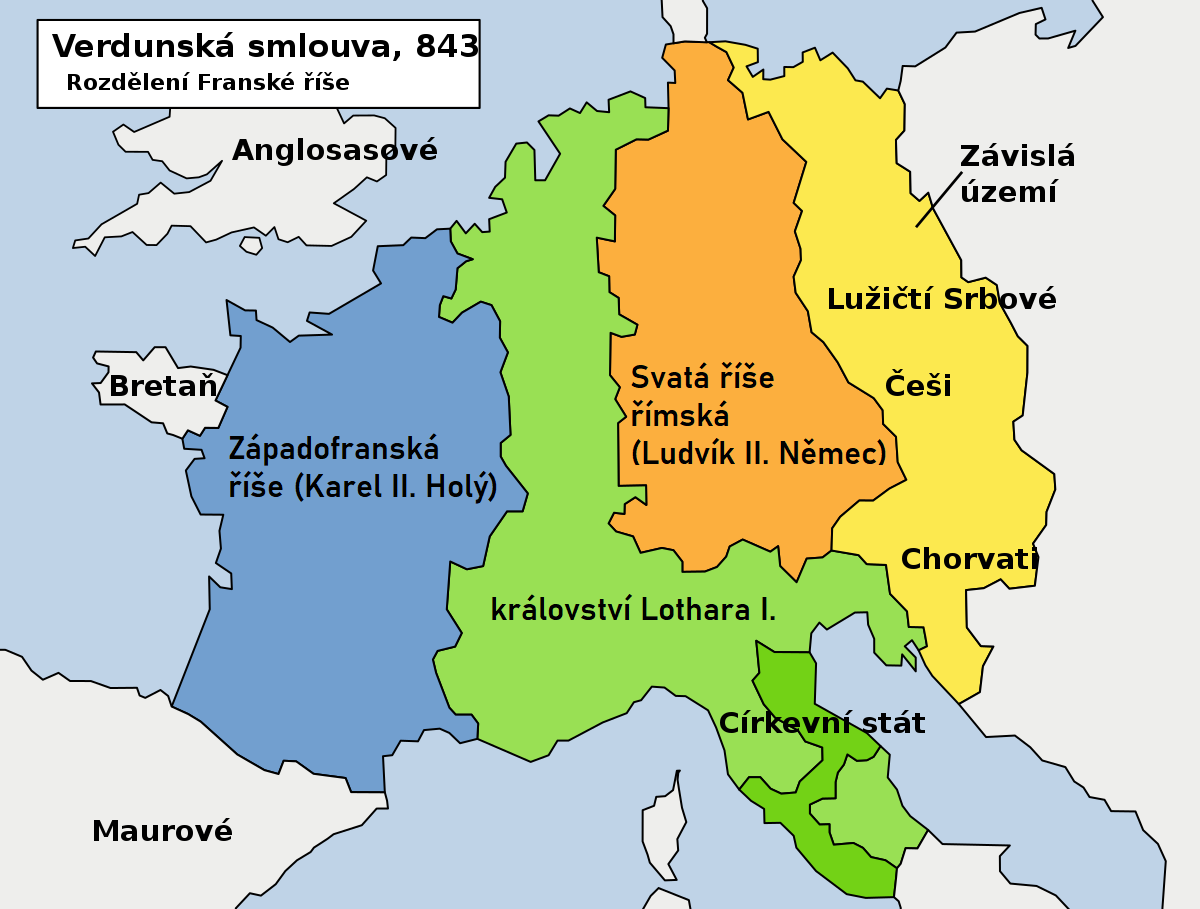
\includegraphics[width=\linewidth]{rozdeleni.png}
\end{figure}



\end{document}
